\documentclass[10pt]{beamer}
\mode<presentation>
{
      \usetheme{Singapore}
	\setbeamercovered{transparent}
}

\usepackage[english]{babel}
\usepackage[T1]{fontenc}
\usepackage{graphicx}
\usepackage{listings}
\usepackage{xcolor}

\lstset{
	basicstyle=\ttfamily\scriptsize,
	breaklines=true,
	frame=single,
	backgroundcolor=\color{gray!10},
	language=Python
}

\title{Fixing plots in passagemath}
\author{Your Name}
\institute{\centering
\includegraphics[width=0.2\textwidth]{math_logo.png}}
\date{\scriptsize Davis Math Lab Presentation\\ May 20--21, 2026}

\begin{document}
	\maketitle

	\begin{frame}{Plots didn't render}
		In Colab, plots showed up as text:
		\vspace{1em}
		\begin{center}
		\texttt{Graphics object consisting of 1 graphics primitive}
		\end{center}
		\vspace{1em}
		You had to patch it yourself in every notebook.
	\end{frame}

	\begin{frame}[fragile]{The workaround}
		\begin{lstlisting}
from io import BytesIO
from matplotlib.backends.backend_agg import FigureCanvasAgg
from sage.plot.graphics import Graphics

def _graphics_repr_png(self):
    figure = self.matplotlib()
    figure.set_canvas(FigureCanvasAgg(figure))
    buf = BytesIO()
    figure.savefig(buf, format='png')
    return buf.getvalue()

Graphics._repr_png_ = _graphics_repr_png
		\end{lstlisting}
	\end{frame}

	\begin{frame}{The fix: PR \#2351}
		Added \texttt{\_repr\_png\_} directly to \texttt{Graphics}.
		\vspace{1em}
		Now \texttt{plot()} just works.
	\end{frame}

	\begin{frame}[fragile]{sin}
		\begin{columns}
			\begin{column}{0.45\textwidth}
				\begin{lstlisting}
plot(math.sin, 0, 6)
				\end{lstlisting}
			\end{column}
			\begin{column}{0.55\textwidth}
				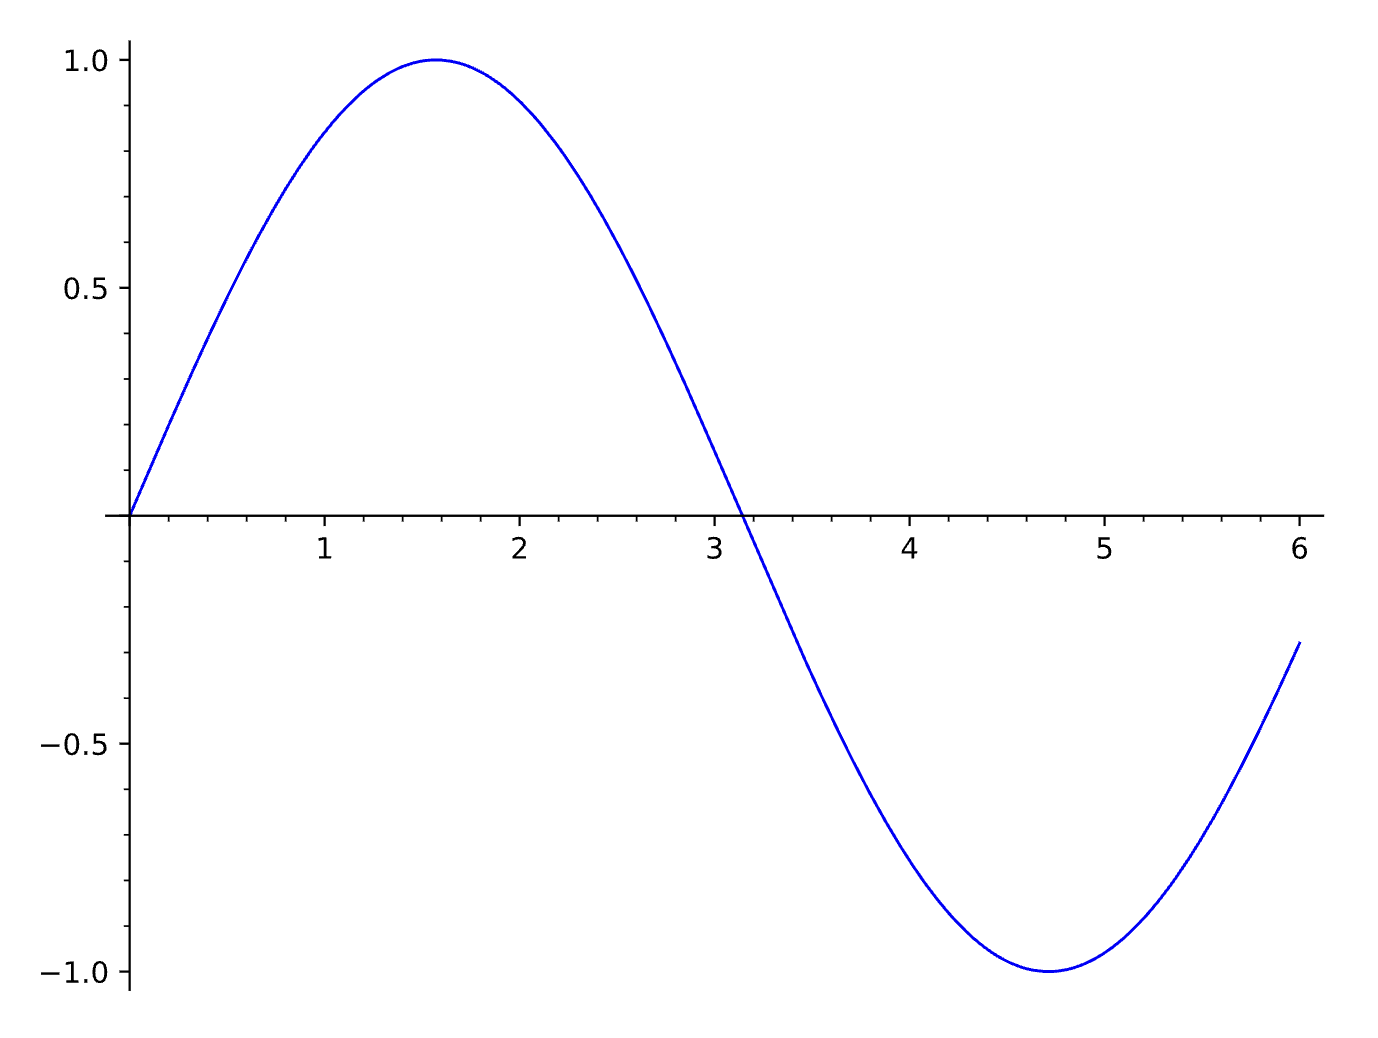
\includegraphics[width=\textwidth]{screenshot_sin.png}
			\end{column}
		\end{columns}
	\end{frame}

	\begin{frame}[fragile]{Linear programming}
		\begin{columns}
			\begin{column}{0.45\textwidth}
				\begin{lstlisting}
A = ([3, 2], [1, 2])
b = (12, 8)
c = (2, 3)
P = InteractiveLPProblem(
    A, b, c, ["x1", "x2"],
    variable_type=">=")
P.plot()
				\end{lstlisting}
			\end{column}
			\begin{column}{0.55\textwidth}
				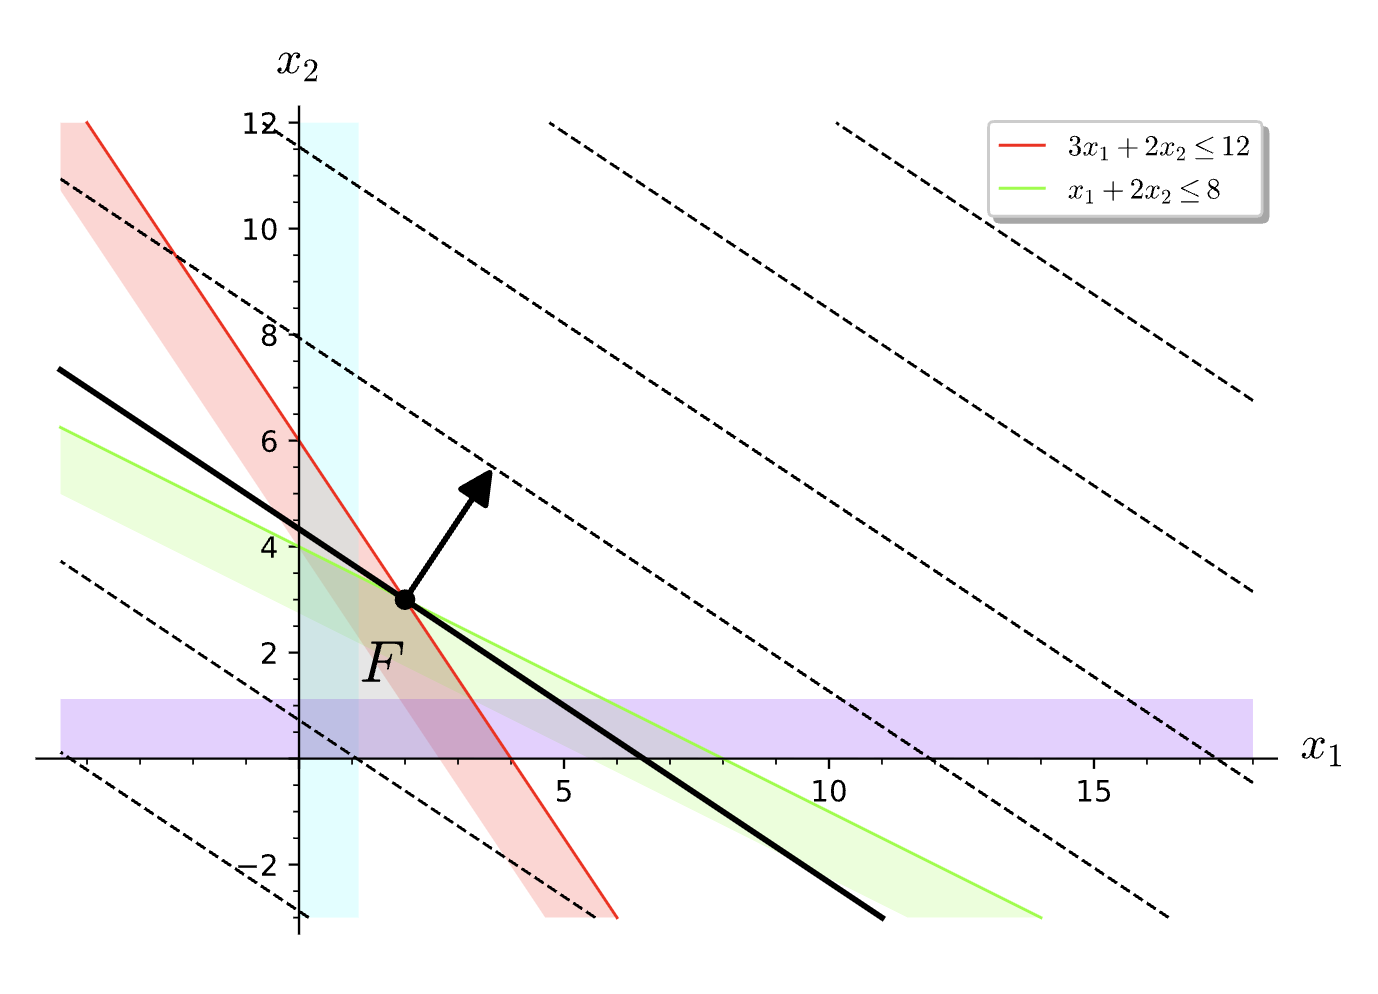
\includegraphics[width=\textwidth]{screenshot_lp.png}
			\end{column}
		\end{columns}
	\end{frame}

	\begin{frame}[fragile]{Queen graph}
		\begin{columns}
			\begin{column}{0.45\textwidth}
				\begin{lstlisting}
G = QueenGraph([3, 3])
G.plot()
				\end{lstlisting}
			\end{column}
			\begin{column}{0.55\textwidth}
				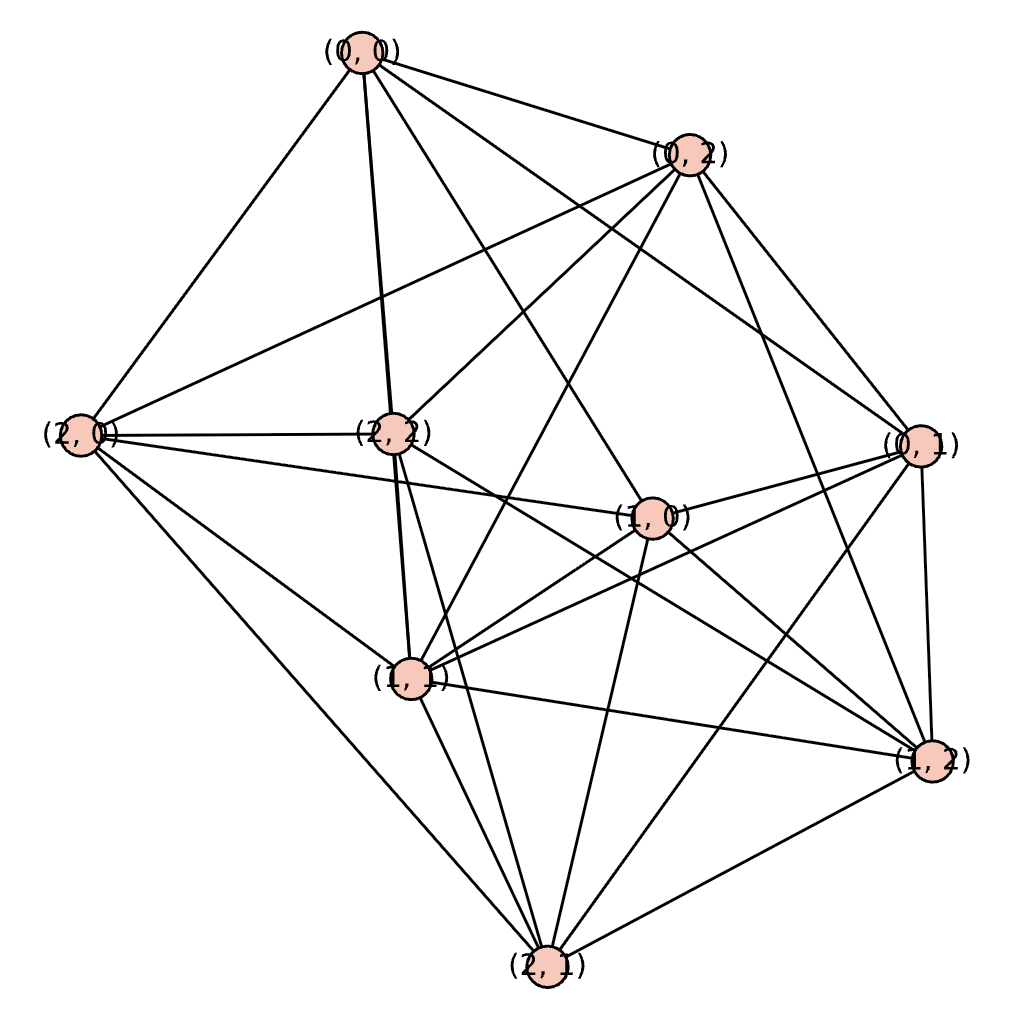
\includegraphics[width=\textwidth]{screenshot_queen.png}
			\end{column}
		\end{columns}
	\end{frame}

\end{document}
